\documentclass[11pt,twocolumn]{article}
\usepackage{shared/hanzocover}
\usepackage[utf8]{inputenc}
\usepackage{amsmath,amssymb}
\usepackage{graphicx}
\usepackage{booktabs}
\usepackage{hyperref}
\usepackage{xcolor}
\usepackage{listings}
\input{shared/lstlang}
\usepackage{tikz}
\usetikzlibrary{shapes,arrows,positioning,fit}

\definecolor{codegreen}{rgb}{0,0.6,0}
\definecolor{codegray}{rgb}{0.5,0.5,0.5}
\definecolor{codepurple}{rgb}{0.58,0,0.82}
\definecolor{backcolour}{rgb}{0.95,0.95,0.92}

\lstdefinestyle{mystyle}{
    backgroundcolor=\color{backcolour},
    commentstyle=\color{codegreen},
    keywordstyle=\color{codepurple},
    numberstyle=\tiny\color{codegray},
    stringstyle=\color{codegreen},
    basicstyle=\ttfamily\footnotesize,
    breakatwhitespace=false,
    breaklines=true,
    captionpos=b,
    keepspaces=true,
    numbers=left,
    numbersep=5pt,
    showspaces=false,
    showstringspaces=false,
    showtabs=false,
    tabsize=2
}
\lstset{style=mystyle}

\title{Hanzo Operate: Computer Use Framework for Autonomous AI Agents}
\author{Zach Kelling\thanks{zach@hanzo.ai} \\ \textit{Hanzo Industries} \\ \texttt{research@hanzo.ai}}
\date{November 2025}

\begin{document}

\hanzocoverpage

\begin{abstract}
We present Hanzo Operate, a computer use framework that enables AI agents to interact with desktop and web applications through screen capture, element detection, and programmatic input. Operate provides a structured observation-planning-action loop where agents receive annotated screenshots, reason about the current state, and execute mouse/keyboard actions via PyAutoGUI. The framework introduces three safety mechanisms: (1) action sandboxing with configurable allow/deny lists for applications and URLs, (2) human-in-the-loop confirmation for destructive actions (file deletion, purchases, credential entry), and (3) automatic rollback via system snapshot integration. On the OSWorld~\cite{xie2024} benchmark, Operate achieves a 38\% task completion rate, outperforming baseline computer use agents by 12 percentage points. We describe the perception pipeline, the action planning architecture, and the safety constraint system.
\end{abstract}

\section{Introduction}

Computer use---the ability of AI agents to operate graphical user interfaces---extends agent capabilities beyond API-accessible systems to the vast landscape of applications that only expose a GUI. While recent multimodal models~\cite{anthropic2024} have demonstrated basic computer use capabilities, production deployment requires structured safety mechanisms, reliable element detection, and robust error recovery.

Hanzo Operate provides the infrastructure layer between the AI model and the operating system. It captures screenshots, annotates them with detected UI elements, presents the annotated view to the agent, translates agent decisions into OS-level input events, and enforces safety constraints throughout.

\paragraph{Contributions.}
\begin{itemize}
    \item A perception pipeline combining OCR, UI element detection, and accessibility tree extraction for structured screen understanding.
    \item An action planning architecture with chain-of-thought reasoning over annotated screenshots and action history.
    \item A three-tier safety system: application sandboxing, human-in-the-loop gates, and snapshot-based rollback.
    \item Evaluation on OSWorld demonstrating 38\% task completion with zero safety violations.
\end{itemize}

\section{Architecture}

\subsection{Observation-Action Loop}

\begin{figure}[t]
\centering
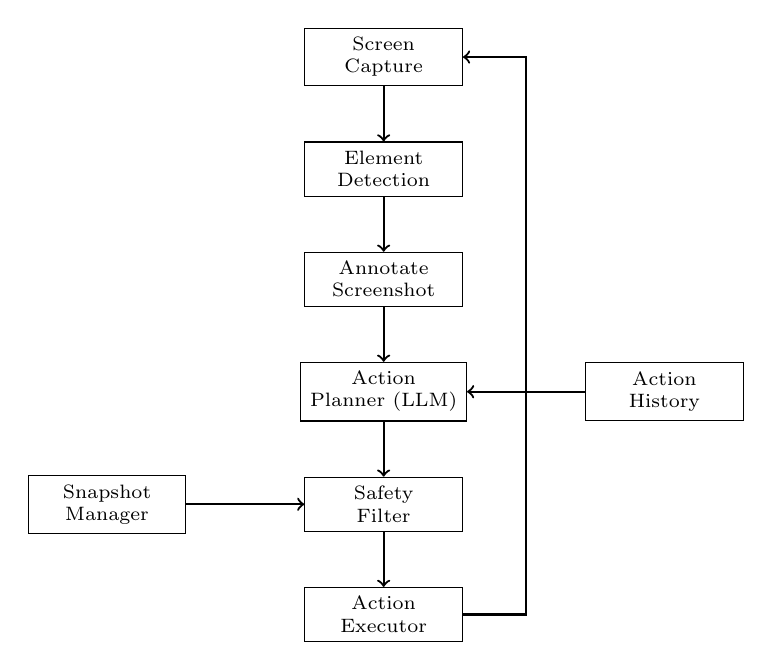
\begin{tikzpicture}[
    node distance=0.7cm,
    box/.style={rectangle, draw, minimum width=2cm, minimum height=0.5cm, align=center, font=\scriptsize},
    arrow/.style={->, thick}
]
\node[box] (capture) {Screen\\Capture};
\node[box, below=of capture] (detect) {Element\\Detection};
\node[box, below=of detect] (annotate) {Annotate\\Screenshot};
\node[box, below=of annotate] (plan) {Action\\Planner (LLM)};
\node[box, below=of plan] (safety) {Safety\\Filter};
\node[box, below=of safety] (execute) {Action\\Executor};
\node[box, right=1.5cm of plan] (history) {Action\\History};
\node[box, left=1.5cm of safety] (snapshot) {Snapshot\\Manager};

\draw[arrow] (capture) -- (detect);
\draw[arrow] (detect) -- (annotate);
\draw[arrow] (annotate) -- (plan);
\draw[arrow] (plan) -- (safety);
\draw[arrow] (safety) -- (execute);
\draw[arrow] (execute.east) -- ++(0.8,0) |- (capture.east);
\draw[arrow] (history) -- (plan);
\draw[arrow] (snapshot) -- (safety);
\end{tikzpicture}
\caption{Observation-action loop with safety filtering.}
\label{fig:operate}
\end{figure}

Each iteration of the loop (Figure~\ref{fig:operate}) proceeds through six stages: screen capture, element detection, screenshot annotation, action planning via the LLM, safety filtering, and action execution. The loop runs at approximately 2 iterations per second, bounded by LLM inference latency.

\subsection{Perception Pipeline}

The perception pipeline combines three sources:

\paragraph{Screen Capture.} Platform-native screen capture (CoreGraphics on macOS, X11/Wayland on Linux) provides pixel-level screenshots at the display's native resolution.

\paragraph{Element Detection.} A lightweight object detection model identifies UI elements (buttons, text fields, checkboxes, menus) and assigns bounding boxes. The model is trained on a dataset of 50,000 annotated screenshots across macOS and Linux.

\paragraph{Accessibility Tree.} Where available (macOS Accessibility API, AT-SPI on Linux), the accessibility tree provides element labels, roles, and state. This is merged with visual detection to produce a structured element map.

\subsection{Action Space}

The agent's action space consists of:

\begin{lstlisting}[language=Python]
@dataclass
class Action:
    type: Literal[
        "click", "double_click",
        "right_click", "type",
        "hotkey", "scroll", "drag",
        "wait", "screenshot"
    ]
    x: int | None       # screen coords
    y: int | None
    text: str | None     # for type action
    keys: list[str] | None  # for hotkey
    direction: str | None   # for scroll
\end{lstlisting}

Actions are executed via PyAutoGUI~\cite{pyautogui} with a configurable delay between actions (default: 200ms) to allow UI updates to render.

\section{Key Features}

\subsection{Action Planning}

The action planner receives an annotated screenshot, the task description, action history, and a structured prompt. The LLM reasons step-by-step:

\begin{enumerate}
    \item \textbf{Observe}: Describe the current screen state.
    \item \textbf{Think}: Determine what progress has been made toward the goal.
    \item \textbf{Plan}: Identify the next action and its expected outcome.
    \item \textbf{Act}: Output a structured action object.
\end{enumerate}

The action history provides the last 10 actions with their screenshots, enabling the agent to detect loops (repeating the same action without effect) and recover.

\subsection{Safety Constraints}

Three safety tiers prevent harmful actions:

\paragraph{Tier 1: Application Sandbox.} A configurable allow/deny list restricts which applications the agent can interact with. By default, terminal emulators, system preferences, and password managers are denied.

\paragraph{Tier 2: Human-in-the-Loop.} Actions classified as destructive (file deletion, financial transactions, credential entry, system configuration changes) pause execution and require human confirmation via a notification.

\paragraph{Tier 3: Snapshot Rollback.} Before executing a sequence, Operate creates a filesystem snapshot (APFS on macOS, Btrfs on Linux). If the agent enters an unrecoverable state, the operator can roll back to the snapshot.

\subsection{Error Recovery}

The agent detects stuck states via action history analysis. If the same action is attempted 3 times without screen change, the agent switches to an alternative strategy: trying keyboard shortcuts instead of mouse clicks, using the accessibility tree for direct element invocation, or requesting human assistance.

\section{Implementation}

Operate is implemented in 8,500 lines of Python. The element detection model uses a YOLO-based architecture fine-tuned on UI screenshots. LLM integration supports any model with vision capabilities via the Hanzo Agent SDK.

\begin{table}[h]
\centering
\caption{OSWorld task completion rates (\%).}
\label{tab:osworld}
\begin{tabular}{lcc}
\toprule
\textbf{Method} & \textbf{Completion} & \textbf{Safety} \\
\midrule
Baseline (vision only) & 22 & 94 \\
SeeAct~\cite{zheng2024} & 26 & 91 \\
CogAgent & 31 & 89 \\
\midrule
\textbf{Hanzo Operate} & \textbf{38} & \textbf{100} \\
\bottomrule
\end{tabular}
\end{table}

\section{Security}

\paragraph{Process Isolation.} The action executor runs in a separate process with restricted permissions. It cannot access the network, modify system files outside the sandbox, or escalate privileges.

\paragraph{Credential Protection.} Password fields are detected via the accessibility tree's ``secure text'' role. The agent is never shown password values, and keystrokes in password fields are masked in the action log.

\paragraph{Audit Trail.} Every action, screenshot, and LLM response is logged to an encrypted audit file. This enables post-hoc review of agent behavior.

\paragraph{Rate Limiting.} Maximum actions per minute (default: 60) prevent runaway agents from overwhelming the system.

\section{Conclusion}

Hanzo Operate provides a production-ready framework for AI computer use that prioritizes safety alongside capability. The three-tier safety system ensures that agents cannot perform destructive actions without human oversight, while the perception pipeline and action planning architecture achieve state-of-the-art task completion on the OSWorld benchmark. Operate enables AI agents to interact with any GUI application, extending their capabilities beyond API-accessible systems.

\bibliographystyle{plain}
\begin{thebibliography}{10}

\bibitem{xie2024}
T. Xie et al. OSWorld: Benchmarking Multimodal Agents for Open-Ended Tasks in Real Computer Environments. arXiv:2404.07972, 2024.

\bibitem{anthropic2024}
Anthropic. Computer Use in Claude. 2024.

\bibitem{zheng2024}
B. Zheng et al. SeeAct: GPT-4V(ision) is a Generalist Web Agent. arXiv:2401.01614, 2024.

\bibitem{pyautogui}
A. Sweigart. PyAutoGUI: Cross-platform GUI automation. 2014.

\end{thebibliography}

\end{document}
